% ============================================================
% S01 — Titre
% ============================================================
\begin{frame}[plain,noframenumbering]
  \titlepage
  \begin{tikzpicture}[remember picture,overlay]
    \node[anchor=south west,inner sep=0pt]
      at ([xshift=.44\paperwidth,yshift=0.78cm]current page.south west)
      {
\includegraphics[height=0.85cm]{media/epita_logo.png}};
  \end{tikzpicture}
\end{frame}

% ============================================================
% S02 — Introduction / accroche (notée)
% ============================================================
\begin{frame}{L'IA se trompe avec aplomb}
  \framesubtitle{Pourquoi la fiabilité est devenue le vrai sujet}
  \begin{columns}[T,onlytextwidth]
    \column{0.46\textwidth}
      \centering
      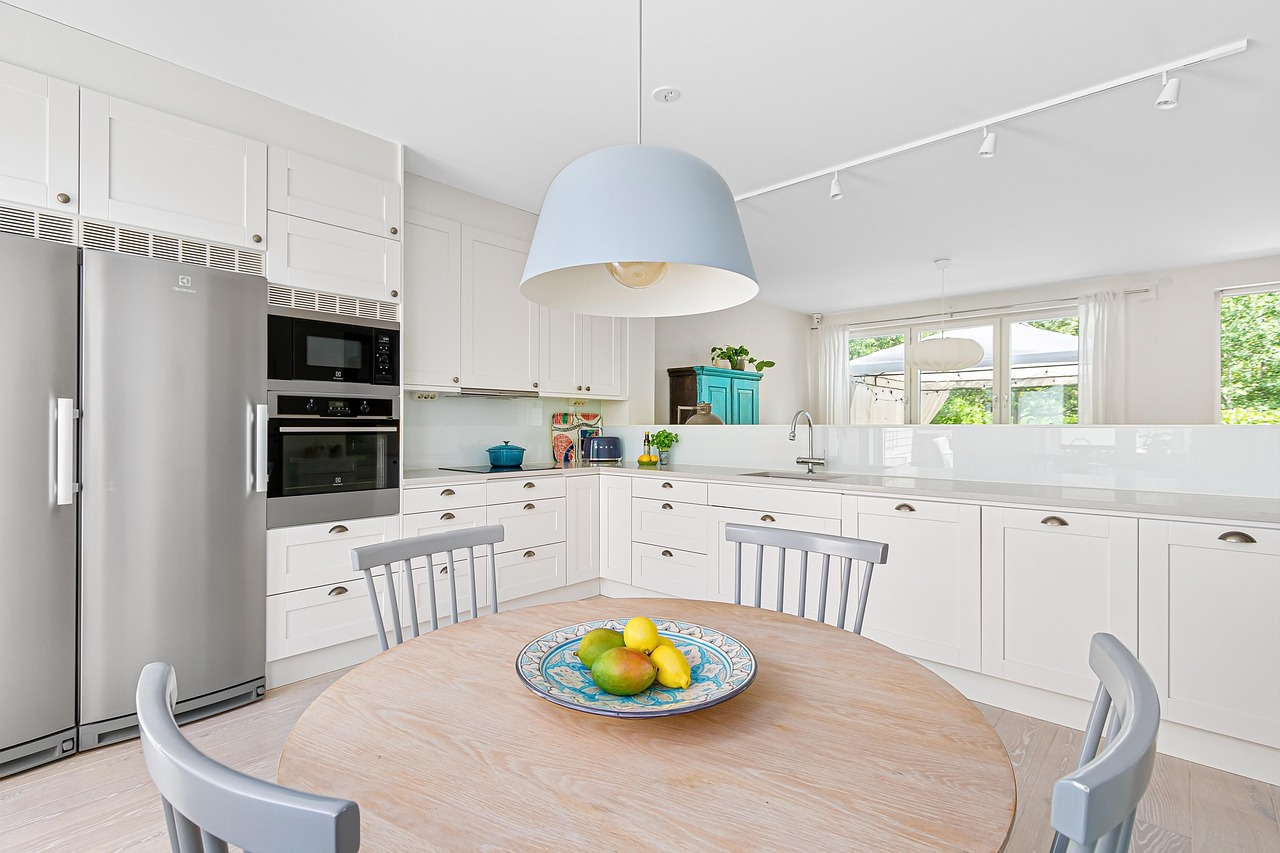
\includegraphics[width=\linewidth,height=0.46\textheight,keepaspectratio]{media/kitchen.png}
      \par\vspace{0.25cm}
      {\scriptsize\color{AubaySlate} Description générée par un VLM (modèle de vision-langage) :\par}
      \vspace{0.14cm}
      {« Un plat bleu avec des fruits, notamment \textcolor{AubayDanger}{\textbf{des pommes et une orange}}\ldots »\par}
    \column{0.50\textwidth}
      \vspace{0.5cm}
      \begin{itemize}
        \item Hallucination visuelle $=$ décrire \textbf{ce qui n'est pas dans l'image}
      \end{itemize}
      \vspace{0.6cm}
      \AubayFocusPanel{Ma mission}{\small Rendre les VLM \textbf{auditables}, \textbf{sans réentraîner} le modèle :}
      \vspace{0.3cm}
      \centering
      \AubayStatusChip{AubayOrange}{DÉTECTER}\hspace{0.2cm}
      \AubayStatusChip{AubayTeal}{MESURER}\hspace{0.2cm}
      \AubayStatusChip{AubaySuccess}{CORRIGER}
  \end{columns}
\end{frame}
